%% For double-blind review submission, w/o CCS and ACM Reference (max submission space)
\documentclass[sigplan,10pt,review,anonymous]{acmart}\settopmatter{printfolios=true,printccs=false,printacmref=false}
%% For double-blind review submission, w/ CCS and ACM Reference
%\documentclass[sigplan,review,anonymous]{acmart}\settopmatter{printfolios=true}
%% For single-blind review submission, w/o CCS and ACM Reference (max submission space)
%\documentclass[sigplan,review]{acmart}\settopmatter{printfolios=true,printccs=false,printacmref=false}
%% For single-blind review submission, w/ CCS and ACM Reference
%\documentclass[sigplan,review]{acmart}\settopmatter{printfolios=true}
%% For final camera-ready submission, w/ required CCS and ACM Reference
%\documentclass[sigplan]{acmart}\settopmatter{}

% Use the postscript times font!
\usepackage{times}
\usepackage{soul}
\usepackage{url}
\usepackage[hidelinks]{hyperref}

\usepackage[utf8]{inputenc}
\usepackage[english]{babel}
\usepackage[small]{caption}

%%%%%%
\newtheorem{theorem}{Theorem}

% Math notation
\RequirePackage[group-separator={,}]{siunitx}
\newcommand{\na}{$\mathrm{N.A.}$}
\newcommand{\minus}{\scalebox{0.7}[1.0]{$-$}}
\newcommand{\expn}[1]{\!\!\times\!\!10^{\minus#1}}
\newcommand{\pval}[2]{$p\textrm{-value} = #1\expn{#2}$}
\newcommand{\set}[1]{\{{}#1\}}
\newcommand{\A}[1]{\mathcal{A}_{#1}}
\newcommand{\N}[1]{n_{#1}(j)}



%%%%%%
\usepackage{float}
\usepackage{listings}
\usepackage{caption}
\usepackage{graphicx}
\usepackage{subcaption}
\usepackage{colortbl}
\usepackage{amsmath}
%\usepackage{amsthm} 
\usepackage{mathpartir}
\usepackage{fancyvrb}\fvset{fontsize=\small}
\usepackage{xspace}
\usepackage{xcolor}
\usepackage{balance}
\usepackage{wrapfig}
\usepackage{multirow}
\usepackage{pifont}
\usepackage{amssymb}
%%%%%%%%%%%%%%%%%%% this can reduce space quite a lot
\usepackage{soul}
\usepackage{microtype}
\usepackage[T1]{fontenc}
\usepackage{dsfont}
%%%%%%%%%%%%%%%%%%% this can reduce space quite a lot
\usepackage{relsize}
\usepackage{tikz}
\usepackage{longtable}
\usepackage{booktabs}
\usepackage{marvosym} 
\usepackage{framed}
\usepackage{mdwlist}
\usepackage{tabularx}
\usepackage{wrapfig}

\usepackage{array}
\usepackage{mathtools}
\usepackage{url}
\usepackage{color}

%% Colors
\definecolor{bgBlock}{rgb}{0.22,0.15,0.49}
\definecolor{bgBlockAlert}{rgb}{0.99,0.84,0.31}
\definecolor{fgBlockAlert}{rgb}{0.22,0.15,0.49}
\definecolor{fgBlock}{rgb}{0.99,0.84,0.31}
\definecolor{darkred}{rgb}{0.5,0,0}
\definecolor{darkgreen}{rgb}{0,0.5,0}
\definecolor{darkblue}{rgb}{0,0,0.5}
\definecolor{Gray}{gray}{0.9}

%%%%%%%%%% added by sofia
\usepackage{algpseudocode}
\usepackage{algorithm}
\usepackage{enumitem}


\usepackage{bm}
\usepackage{cleveref}
\usepackage{textcomp}
\usepackage{pdfpages}
\usepackage{chngpage}


%\usepackage[hyphenbreaks]{breakurl}


%%%%%%%%%%

\usepackage[most]{tcolorbox}
\newtcolorbox{myframe}[1][]{
	enhanced,
	arc=0pt,
	outer arc=0pt,
	colback=white,
	boxrule=0.5pt,
	boxsep=1pt,left=3pt,right=3pt,top=5pt,bottom=5pt,
	fontupper=\small,
	size=small
	#1
}

%%%%%%%%%%
% appendix 
\usepackage[toc,page]{appendix}
\usepackage{makecell}


%%%%% Theorem -> Claim

\newtheorem{thm}{Theorem} % the main one
\newtheorem{lemma}[thm]{Lemma}

\newcommand{\thistheoremname}{}
\newtheorem{genericthm}[thm]{\thistheoremname}
\newenvironment{namedthm}[1]
  {\renewcommand{\thistheoremname}{#1}
   \begin{genericthm}}
  {\end{genericthm}}





\newcommand{\Fix}[1]{\textbf{[[}{\color{red} #1}\textbf{]]}}
\newcommand{\Anonim}[2]{#1}
\newcommand{\ie}{i.e.}
\newcommand{\eg}{e.g.}
\newcommand{\cf}{cf.}
\newcommand{\etal}{et al.}
\newcommand{\comments}[1]{}
\newcommand{\varex}{\textsc{Varex}}
\newcommand{\tsig}{OUR}
\newcommand{\tnamepar}[1]{\tname{}\texttt{[#1]}}
\newcommand{\CodeIn}[1]{{\small\texttt{#1}}}
\newcommand{\pw}{\textsc{pw}}
\newcommand{\pwopt}{\textsc{pw-opt}}
\newcommand{\dd}{\CodeIn{DD}}
\newcommand{\acrAbrev}{APR}
\newcommand{\RQ}{RQ}
\newcommand{\morpho}{\emph{morpho}}
\newcommand{\lithium}{\emph{lithium-slicer}}
\newcommand{\success}{\leavevmode\color[HTML]{009901}}

\definecolor{bs}{rgb}{0.59, 0.0, 0.09}
\definecolor{d}{HTML}{800000}

\newcommand{\BS}[1]{\textbf{[BS:[}{\color{bs} #1}\textbf{]]}}
\newcommand{\Mar}[1]{\textbf{[Marcelo:[}{\color{orange} #1}\textbf{]]}}
\newcommand{\Sof}[1]{\textbf{[Sofia:[}{\color{cyan} #1}\textbf{]]}}
\newcommand{\oururl}{\Fix{url here}}
\newcommand{\tname}{\Fix{Critical Slicing Revisited}}

\newcommand{\numPrograms}{six}
\newcommand{\numFaults}{395}
\newcommand{\topk}{top-$k$}

\newcommand{\sfl}{SFL}
\newcommand{\CS}{CS}
\newcommand{\cs}{CS}
\newcommand{\ds}{DS}
\newcommand{\dfj}{Defects4J}
\newcommand{\orbs}{ORBS}
\newcommand{\comb}{\sfl{}+\ds{}}
\newcommand{\apr}{APR}

%% subject names as in https://github.com/rjust/defects4j
\newcommand{\chart}{JFreechart}
\newcommand{\closure}{Closure compiler}
\newcommand{\lang}{Apache commons-lang}
\newcommand{\cmath}{Apache commons-math}
\newcommand{\mockito}{Mockito}
\newcommand{\jtime}{Joda-Time}

\newcommand{\cmark}{\ding{51}}%
\newcommand{\xmark}{\ding{55}}%


%% Conference information
%% Supplied to authors by publisher for camera-ready submission;
%% use defaults for review submission.
\acmConference[PL'18]{ACM SIGPLAN Conference on Programming Languages}{January 01--03, 2018}{New York, NY, USA}
\acmYear{2018}
\acmISBN{} % \acmISBN{978-x-xxxx-xxxx-x/YY/MM}
\acmDOI{} % \acmDOI{10.1145/nnnnnnn.nnnnnnn}
\startPage{1}

%% Copyright information
%% Supplied to authors (based on authors' rights management selection;
%% see authors.acm.org) by publisher for camera-ready submission;
%% use 'none' for review submission.
\setcopyright{none}
%\setcopyright{acmcopyright}
%\setcopyright{acmlicensed}
%\setcopyright{rightsretained}
%\copyrightyear{2018}           %% If different from \acmYear

%% Bibliography style
\bibliographystyle{ACM-Reference-Format}
%% Citation style
%\citestyle{acmauthoryear}  %% For author/year citations
%\citestyle{acmnumeric}     %% For numeric citations
%\setcitestyle{nosort}      %% With 'acmnumeric', to disable automatic
                            %% sorting of references within a single citation;
                            %% e.g., \cite{Smith99,Carpenter05,Baker12}
                            %% rendered as [14,5,2] rather than [2,5,14].
%\setcitesyle{nocompress}   %% With 'acmnumeric', to disable automatic
                            %% compression of sequential references within a
                            %% single citation;
                            %% e.g., \cite{Baker12,Baker14,Baker16}
                            %% rendered as [2,3,4] rather than [2-4].


%%%%%%%%%%%%%%%%%%%%%%%%%%%%%%%%%%%%%%%%%%%%%%%%%%%%%%%%%%%%%%%%%%%%%%
%% Note: Authors migrating a paper from traditional SIGPLAN
%% proceedings format to PACMPL format must update the
%% '\documentclass' and topmatter commands above; see
%% 'acmart-pacmpl-template.tex'.
%%%%%%%%%%%%%%%%%%%%%%%%%%%%%%%%%%%%%%%%%%%%%%%%%%%%%%%%%%%%%%%%%%%%%%

\begin{document}

%% Title information
\title{The Impact of Critical Slicing in SFL\Comment{tatistical Fault Localization}}         %% [Short Title] is optional;
                                        %% when present, will be used in
                                        %% header instead of Full Title.
%\titlenote{with title note}             %% \titlenote is optional;
                                        %% can be repeated if necessary;
                                        %% contents suppressed with 'anonymous'
%\subtitle{Subtitle}                     %% \subtitle is optional
%\subtitlenote{with subtitle note}       %% \subtitlenote is optional;
                                        %% can be repeated if necessary;
                                        %% contents suppressed with 'anonymous'


%% Author information
%% Contents and number of authors suppressed with 'anonymous'.
%% Each author should be introduced by \author, followed by
%% \authornote (optional), \orcid (optional), \affiliation, and
%% \email.
%% An author may have multiple affiliations and/or emails; repeat the
%% appropriate command.
%% Many elements are not rendered, but should be provided for metadata
%% extraction tools.

%% Author with single affiliation.
\author{First1 Last1}
\authornote{with author1 note}          %% \authornote is optional;
                                        %% can be repeated if necessary
\orcid{nnnn-nnnn-nnnn-nnnn}             %% \orcid is optional
\affiliation{
  \position{Position1}
  \department{Department1}              %% \department is recommended
  \institution{Institution1}            %% \institution is required
  \streetaddress{Street1 Address1}
  \city{City1}
  \state{State1}
  \postcode{Post-Code1}
  \country{Country1}                    %% \country is recommended
}
\email{first1.last1@inst1.edu}          %% \email is recommended

%% Author with two affiliations and emails.
\author{First2 Last2}
\authornote{with author2 note}          %% \authornote is optional;
                                        %% can be repeated if necessary
\orcid{nnnn-nnnn-nnnn-nnnn}             %% \orcid is optional
\affiliation{
  \position{Position2a}
  \department{Department2a}             %% \department is recommended
  \institution{Institution2a}           %% \institution is required
  \streetaddress{Street2a Address2a}
  \city{City2a}
  \state{State2a}
  \postcode{Post-Code2a}
  \country{Country2a}                   %% \country is recommended
}
\email{first2.last2@inst2a.com}         %% \email is recommended
\affiliation{
  \position{Position2b}
  \department{Department2b}             %% \department is recommended
  \institution{Institution2b}           %% \institution is required
  \streetaddress{Street3b Address2b}
  \city{City2b}
  \state{State2b}
  \postcode{Post-Code2b}
  \country{Country2b}                   %% \country is recommended
}
\email{first2.last2@inst2b.org}         %% \email is recommended


%% Abstract
%% Note: \begin{abstract}...\end{abstract} environment must come
%% before \maketitle command
\begin{abstract}
Text of abstract \ldots.
\end{abstract}


%% 2012 ACM Computing Classification System (CSS) concepts
%% Generate at 'http://dl.acm.org/ccs/ccs.cfm'.
\begin{CCSXML}
<ccs2012>
<concept>
<concept_id>10011007.10011006.10011008</concept_id>
<concept_desc>Software and its engineering~General programming languages</concept_desc>
<concept_significance>500</concept_significance>
</concept>
<concept>
<concept_id>10003456.10003457.10003521.10003525</concept_id>
<concept_desc>Social and professional topics~History of programming languages</concept_desc>
<concept_significance>300</concept_significance>
</concept>
</ccs2012>
\end{CCSXML}

\ccsdesc[500]{Software and its engineering~General programming languages}
\ccsdesc[300]{Social and professional topics~History of programming languages}
%% End of generated code


%% Keywords
%% comma separated list
\keywords{keyword1, keyword2, keyword3}  %% \keywords are mandatory in final camera-ready submission


%% \maketitle
%% Note: \maketitle command must come after title commands, author
%% commands, abstract environment, Computing Classification System
%% environment and commands, and keywords command.
\maketitle

\section{Introduction}

%% PROBLEM MOTIVATION
Automated debugging is very important.\Fix{...elaborate...}

Statistical Fault Localization (\sfl{}) and Dynamic Slicing are
popular complementary approaches proposed to automate debugging.
\sfl{}~\cite{7390282} computes
suspiciousness values associated with program entities (e.g., basic
blocks) using coverage information of passing and failing test
cases. \sfl{} produces a list of program entities ranked in
decreasing order of suspiciousness.  \sfl{} received tremendous
attention over the years, but its applicability to support debugging
remains
questionable~\cite{ang-perez-van-deursen-rui-2017,Pearson:2017:EIF:3097368.3097441,Xie:2016:RAD:2884781.2884834}.
Despite the skepticism of the research community, \sfl{} has been shown
useful in supporting downstream analyses, such as Automated Program Repair
(\apr{})~\cite{automatic-software-repair-survey2017,kim-etal-daghstul2017},
an increasingly popular technique that looks for likely fixes to
likely buggy statements.  Tools like JAFF \cite{arcuri-2011}, Prophet
\cite{long-rinard-2016}, SemFix \cite{nguyen-qi-roychoudhury-2013},
and SPR \cite{long-rinard-2015} use \sfl{} to guide the search for
likely fixes. Dynamic Slicing~\cite{Agrawal:1990:DPS:93542.93576} is another popular
technique for automated debugging. It takes as input a failing test
and produces on output a set of statements--the slice--that influence
the evaluation of the fault-revealing assertion.

%Recent \apr{} techniques use \sfl{} to guide
%the search for repairs .

%% \Fix{Revise this $\rightarrow$} Mao and Wang
%% \cite{lei-mao-dai-wang-2012} had promising results compared to \sfl{}
%% state of the art techniques, such as Tarantula [cite] and Ochiai
%% [cite], concerning the relative percentage of the code above the
%% fault. Prior work used the same measurement approach
%% \cite{santelices-jones-yu-harrold-2009,wang-cheung-chan-zhang-2009,jones-2005}.
%% However, the problem with this approach lies in the effort to find the
%% defect, as shown on Parnin and Orso's study \cite{parnin-orso-2011},
%% in which a percentage rank does not scale with the size of a
%% codebase. For example, if a fault statement is ranked on the 83rd
%% position as a result of a \sfl{} technique, the percentage rank using
%% a codebase of 8300 LOC is only 1\%, with the amount of absolute lines
%% of code to be examined not being considered.  This can result in
%% millions of lines of code to be analysed, proving that a percentage
%% rank is not a practical evaluation metric
%% \cite{ang-perez-van-deursen-rui-2017}.  \Fix{end here}



This paper reports the results of an empirical study to evaluate the
impact of Dynamic Slicing (\ds{}) to improve \sfl{}. The intuition for
the \comb{} combination is that several highly ranked statements,
albeit covered by failing executions, may be unrelated to the
fault. Prior work reported promising results in this combination
\cite{Wotawa:2010:FLB:1848650.1849235,Alves:2011:FUD:2190078.2190115,DBLP:conf/ecai/HoferW12,lei-mao-dai-wang-2012}.
For example, Lei \etal{}~\cite{lei-mao-dai-wang-2012} reported a
reduction of 78.3\% in \emph{effort}~\cite{7927959} to analyze
rankings when using dynamic slicing in combination with \sfl{} versus
plain \sfl{}. We found surprising that, despite these findings,
reported nearly 5 years ago, no tool or client analyses use this
combination today. One hypothesis to explain that observation is that
results reported in prior work are not as good as it seems. Prior
research evaluated \sfl{} using relative metrics, based on the
position of the first faulty statements found in the ranking relative
to the total number of ranking statements, which is often a very high
number. Ang \etal~\cite{ang-perez-van-deursen-rui-2017} recently
pointed to that fact encouraging developers to adopt precise metrics
such as top@n
\cite{Wu:2014:CLC:2610384.2610386,Lucia:2014:FFL:2642937.2642983,Wen:2016:LLB:2970276.2970359}. The
goal of this paper is to reassess whether the \comb{} combination is
worthwhile under the light of this metric. Developers of techniques
such as \acrAbrev{} would benefit from these results~---~either to
improve their results or to be aware they should not invest on this
integration.

%% ~\cite{Jin:2013:FFL:2483760.2483763,Laghari:2016:FSB:2970276.2970308,campos-etal-ase2016,DBLP:journals/stvr/LiuLNBB16,DBLP:conf/hvc/LidO16,7589823}

\Fix{Mention the research questions at some point, plus contributions.}

\section{Dynamic Slicing}
\label{sec:slicing}

Program slicing is a program understanding method to identify the
relevant parts of the program with respect to given points of
interest.  This paper focuses on dynamic slicing~--~as opposed to
static slicing~\cite{Weiser:1981:PS:800078.802557}~--~for its
application in automated software
debugging~\cite{Binkley:2014:OLP:2635868.2635893}.  To select a slicer
implementation to run our experiments, we considered two criteria:
robustness as to support non-trivial programs and efficiency as to
support execution of our experiments in reasonable time.
Unfortunately, we failed to find public implementations satisfying
these criteria.

For those reasons, we decided to implement a critical slicer for Java,
which is the language of the subjects in our dataset, \dfj{}. We
focused on Critical Slicing~\cite{DeMillo:1996:CSS:229000.226310} for
its simplicity.\Comment{ In constrast with alternative slicing
  implementations based on dependency
  chains~\cite{Tip:1994:SPS:869354}\Comment{(\eg{},
    JSlice~\cite{Wang:2004:UCB:998675.999455} and
    JavaSlicer~\cite{hammacher-bachthesis-2008})},} Critical Slicing
prescribes a black-box language-semantics-agnostic recipe to computing
executable slices\footnote{In the original implementation, critical
  slicing was not guaranteed to be executable.  Above we refer to the
  basic strategy of deleting statement and checking outcomes.}.
Critical Slicing slices the program by deleting statements such that
the sliced program preserves critical observations (\eg{}, assertion
violations).  The output we used to determine equivalence of the
original failing execution and the sliced failing execution was the
stack trace produced by the assertion violation.  It is important to
note that Binkley \etal{} recently proposed the critical slicer
ORBS~\cite{DBLP:conf/scam/BinkleyGHIKY15}, but its design sacrifies
efficiency (important to run our experiments) for generality. Some of
the slicing jobs we ran on ORBS took hours to run. For example,
\Fix{...elaborate...}

The principle of Critical Slicing is rather simple, consisting of
mutating the program and observing the output. Despite that,
optimizations are important to make a Critical Slicing implementation
efficient. We describe the optimizations we used in the following.

%% \vspace{1ex}\noindent\textbf{Blackbox slicing.} Removing statements
%% from the program is necessary to discover whether it is essential
%% to the execution or not. For that reason, we compare the test stack
%% trace to look for changes in the output. Considering one execution,
%% if one line of the stack trace changes and that change is not
%% related to random values (\eg{}, hashcode), we discard that
%% specific slice. However, not every test case produces a stack trace
%% (\ie{}, passing tests), and thus, we guarantee that the test has
%% executing code by not instrumenting test classes and test methods.

\vspace{1ex}\noindent\textbf{Single compilation.}  Recompilation is a
major cost associated with critical
slicing~\cite{DBLP:conf/scam/BinkleyGHIKY15}. For example, \Fix{...\%
  of time in a slicing job from ORBS is due to compilation}. For that reason, our slicer uses a
program schemata where every statement in function bodies is guarded
by a branch predicate to control its activation. The slicer
re-executes the program with different guard configurations, recording
the smallest slice found. It uses a local search to find the smallest
slice for a given time budget. A slice is encoded as a list of flags,
each indicating whether or not a given guard is active. The initial
configuration of a slicing job has the flags set for all statements
covered by a given test.

%% \vspace{1ex}\noindent\textbf{Structure Awareness.}
%% ORBS is language-agnostic; it removes text from files but it does not
%% parse code. Each removal can lead to malformed
%% code. \Mar{$\leftarrow$how do we deal with this in the bytecode
%%   instrumentation?  explain...} We collect constraints of the form
%% $b\rightarrow{}a$ during code instrumentation to indicate that guard
%% $b$ is used in the region guarded by $a$, reflecting the nested
%% structure of the code. The slicer uses these constraints to prune the
%% search space of guard configurations, encoding the slice. For example,
%% it does not make sense to include statement $b$ in the slice and not
%% including statement $a$.

\vspace{1ex}\noindent\textbf{Clean state execution.} Re-execution of a
given test is necessary in Critical Slicing. However, test
re-execution may introduce flakiness due to side-effects in data
reachable from static fields. One alternative to address this problem
is to run each test in a separate JVM. Unfortunately, that alternative
is prohibitively slow. For that, we ran the slicing job in a single
JVM, using a test runner that is able to clean the static area of the
JVM as follows. At every re-execution of the critical slicer, the test
runner creates a new instance of a custom class loader, child of the
original JVM class loader.  Before loading a class, the custom class
loader checks in a cache whether or not the bytecodes were already
loaded. If not, the class file is loaded from disk and the bytecodes
are stored in the cache for future access. If the bytecodes were
previously loaded, the slicer avoids disk access by reading the data
directly from the cache.  To sum, the use of a new class loader
enables the slicer to ``reset'' the state prior to a new execution of
the same test~---~the objects accessible from the static area become
unreachable when the class loader is disposed at the end of an
execution.

\vspace{1ex}
Our implementation is publicly available under the following link (not
anonymized): \oururl{}.

\section{\sfl}
\label{sec:sfl}

\Mar{borrowed from our ICST17 paper. needs to }

Spectrum-based fault localization is an approach to pinpointing bugs
in software programs~\cite{FLSurvey2016, DBLP:conf/kbse/JonesH05,
  DBLP:journals/smr/LuciaLJTB14, DBLP:journals/jss/AbreuZGG09}.  In
spectrum-based fault localization, the following is given: a finite
set $\mathcal{C} = \set{c_1,c_2,...,c_M}$ of $M$ system
\emph{components}\footnote{A component can be any source code artifact
  of arbitrary granularity such as a class, a method, a statement, or
  a branch~\cite{DBLP:journals/stvr/HarroldRSWY00}.}; a finite set
$\mathcal{T} = \set{t_1,t_2,...,t_N}$ of $N$ system transactions,
which correspond to records of a system execution, such as test cases;
the error vector $e = \set{e_1,e_2,...,e_N}$, where $e_i = 1$ if
transaction $t_i$ has failed and $e_i = 0$ otherwise; and an $N \times
M$ coverage matrix $\mathcal{A}$, where $\A{ij}$ denotes the
coverage of component $c_j$ in transaction $t_i$.
The pair $(\mathcal{A},e)$ is commonly referred to as
spectrum~\cite{DBLP:journals/stvr/HarroldRSWY00}, and is depicted in~\cite{fig:spectrum-example}.
Several types of spectra exist.
The most commonly used is called hit-spectrum, where the coverage matrix is encoded in terms of
binary \emph{hit} (1) and \emph{not hit} (0) flags, i.e.,
$\A{ij} = 1$ if $c_j$ is involved in $t_i$ and $\A{ij} = 0$
otherwise.

\begin{figure}[h!]
    \centering
    \begin{tabular}{c|cccc|c}
      $\mathcal{T}$ & $c_1$    & $c_2$    & $\cdots$ & $c_M$    & $e$    \\ \hline
      $t_1$         & $\A{11}$ & $\A{12}$ & $\cdots$ & $\A{1M}$ & $e_1$  \\
      $t_2$         & $\A{21}$ & $\A{22}$ & $\cdots$ & $\A{2M}$ & $e_2$  \\
      \vdots        & \vdots   & \vdots   & $\ddots$ & \vdots   & \vdots \\
      $t_N$         & $\A{N1}$ & $\A{N2}$ & $\cdots$ & $\A{NM}$ & $e_N$  \\
    \end{tabular}
    \caption{An example spectrum.}
    \label{fig:spectrum-example}
\end{figure}

The pair $(\mathcal{A},e)$ serves as input to the fault localization technique.
With this input, the next step in this coverage-based technique consists of determining what columns
of the matrix $A$ resemble the error vector $e$ the most.
For that, an intermediate component frequency aggregator is computed:
%
\begin{equation}\label{eq:occurrence}
 n_{pq}(j) = |\{i\mid \A{ij}=p \wedge e_i=q\}|
\end{equation}
%
\noindent where $n_{pq}(j)$ is the number of runs in which the
component $j$ has been active during execution ($p = 1$) or not
($p=0$), and in which the runs failed ($q = 1$) or passed ($q = 0$).
For instance, $n_{11}(j)$ counts the number of times component $j$ has
been involved ($p = 1$) in failing executions ($q = 1$), whereas
$n_{10}(j)$ counts the number of times component $j$ has been involved
in passing executions.

We then calculate similarity to the error vector by means of applying \emph{fault predictors} to
each component to produce a score quantifying how likely it is to be faulty.
Components are then ranked according to such likelihood scores and reported to the user.

\section{Dynamic Slicing + \sfl{}}
\label{sec:combination}

The methodology we used to combine dynamic slicing with \sfl{}
consists of the following steps: (1) Compute the execution spectra as
discussed in Section~\ref{sec:sfl}, (2) Compute slices associated with
tests, (3) Adjust the spectra computed in Step 1 with results obtained
in Step 2, and (4) Compute suspiciousness
scores. Figure~\ref{fig:illustration} illustrates the process of
updating the spectra and suspiciousness ranking as result of slicing
the program against the failing test $t_2$.  The faulty statement in
this example is the component $c_2$.

%% \begin{enumerate}
%% \item\label{step-spectra} Compute the execution spectra.
%% \item\label{step-slice} Compute slices associated with tests.
%% \item Adjust the spectra computed in Step~\ref{step-spectra} with
%%   results obtained in Step~\ref{step-slice}.
%% \item Compute suspiciousness scores.
%% %\item {[optional]} Filter statements covered by selected failing tests.
%% \end{enumerate}

\begin{figure}[h!]
  \centering
{\def\arraystretch{0.9}\setlength{\tabcolsep}{3pt}
   \begin{tabular}{c|ccccc|c}
     $\mathcal{T}$ & $c_1$    & $c_2$   & $c_3$ & $c_4$ &  $c_5$   & $e$    \\ \hline
     $t_1$         & 1 & 0 & 1 & 1 & 0 &\cmark  \\
     $t_2$         & 0 & 1 & 1 & 1 & 1 &\xmark  \\
     $t_3$         & 1 & 0 & 1 & 0 & 0 &\xmark  \\
     $t_4$         & 0 & 1 & 0 & 0 & 1 &\cmark  \\
     $t_5$         & 1 & 0 & 0 & 1 & 1 &\cmark \\
     \hline
   \end{tabular}
   \quad
   $\Rightarrow$
   \quad
   \begin{tabular}{c|ccccc|c}
     $\mathcal{T}$ & $c_1$    & $c_2$   & $c_3$ & $c_4$ &  $c_5$   & $e$    \\ \hline
     $t_1$         & 1 & 0 & 1 & 1 & 0 &\cmark  \\
     $t_2$         & 0 & 1 & {\cellcolor{Gray} 0} & {\cellcolor{Gray} 0} & 1 &\xmark  \\
     $t_3$         & 1 & 0 & 1 & 0 & 0 &\xmark  \\
     $t_4$         & 0 & 1 & 0 & 0 & 1 &\cmark  \\
     $t_5$         & 1 & 0 & 0 & 1 & 1 &\cmark  \\
     \hline
   \end{tabular}

   \vspace{3ex}

   \begin{tabular}{cccccc}
     & $c_1$    & $c_2$   & $c_3$ & $c_4$ &  $c_5$  \\
     & 0.32 & 0.35 & 0.55 & 0.59 & 0.32 \\
   \end{tabular}
   \quad
   $\Rightarrow$
   \quad
   \begin{tabular}{cccccc}
     & $c_1$    & $c_2$   & $c_3$ & $c_4$ &  $c_5$  \\
     & 0.32 & 0.35 & {\cellcolor{Gray}0.29} & {\cellcolor{Gray}0.32} & 0.32 \\
   \end{tabular}

 }
\caption{Illustration of spectra and ranking update.}
\label{fig:illustration}
\end{figure}

The slice obtained from $t_2$ is $\{c_2, c_5\}$.  Intuitively, slicing
enables identification of cells in the matrix (/spectra) whose values
can be set to zero. In general, updates in the matrix results in an
increase of suspiciousness for a given component when the target test
is passing or a reduction of suspiciousness when the target test is
failing. Consider the Ochiai formula~\cite{DBLP:conf/prdc/AbreuZG06}

\[
\frac{\N{11}}{\sqrt{\N{11}+\N{01}} + \sqrt{\N{11}+\N{10}}}
\vspace{1ex}\], where $n_{pq}(j)$ is the number of runs in which the
component $j$ has been active during execution ($p = 1$) or not
($p=0$), and in which the runs failed ($q = 1$) or passed ($q = 0$).
Slicing of a failing test reduces the value of $\N{11}$ and increases
the value of $\N{01}$ for those statements $j$ which are not part of
the slice. Therefore, suspiciosness of those statements decrease. In
this example, components $c_3$ and $c_4$, which are not in the slice
of $t_2$, have their suspiciousness reduced, enabling the faulty
component $c_2$ to rise from the third to the first position in the
ranking.


\Fix{I suggest to add an algorithm section and perhaps a discussion on
time/space complexity.}

\section{Evaluation}
\label{sec:eval}

This section reports results of our study to assess the impact of the
\comb{} combination.

\subsection{Objects of Analysis}

Following other recent studies, we used the \dfj{} benchmark in our
experiments~\cite{just-defects4j-issta2014}. The \dfj{} benchmark
includes six subjects and 395 faults.
\lang{} is a library
that provides a set of helper utilities for the {\small\texttt{java.lang}}
API. \cmath{} is a lightweight library of self-contained
mathematics and statistics components. The \closure{} is a toolset for
turning JavaScript files into smaller scripts for faster
download and execution in the browser. \chart{} is a library with a
full-featured charts user interface for Java. \jtime{} is a
lightweight library that aims to replace the default Java
{\small\texttt{java.util.Date}} classes providing simpler APIs. \mockito{} is
a mocking testing framework.\Comment{ that enables the developer to simulate
the behavior of classes that cannot be used in unit testing.}

\newcommand{\cgray}[1]{\cellcolor{gray!25}#1}
\begin{table}[h]
  \centering
  \setlength{\tabcolsep}{4pt}
    \begin{tabular}{lrrr}
      \toprule
      Project            & Size (kLOC) & \# Tests & \# Defects \Comment{& Failing Test Cases &}  \\
      \midrule
      \lang{}            & -  & - & 65          \Comment{& 124   &  -}\\
      \cmath{}           & -  & - & 106          \Comment{& 177   &  -}\\
      \closure{}         & -  & - & 133         \Comment{& 350   &  -}\\
      \chart{}           & -  & - & 26         \Comment{& 92    &  -}\\
      \jtime{}           & -  & - & 27          \Comment{& 76    &  -}\\
      \mockito{}         & -  & - & 38          \Comment{& 118   &  -}\\
      \bottomrule
  \end{tabular}
\caption {Characterization of \dfj{} subjects.}
\end{table}
\normalsize


%% old text related to single faults...
%%%%%%%%%%%%
%% It is important to note that the construction of the \dfj{} dataset is
%% not suited to evaluate the rate of single faults, but prior research
%% did that.  Perez~\etal{}~\cite{7927959} recently showed that single
%% faults are prevalent in open-source project. They conducted a
%% comprehensive empirical study involving 279 open-source Java projects
%% where they found that single faults were observed in 82\% of the cases
%% of regression.


\subsection{Results of Dynamic Slicing}

We describe the results of dynamic slicing alone in the following.



\subsubsection{How much reduction in one execution trace
  can one get with Dynamic Slicing?}

Table~\ref{fig:ds-reduction} shows the average reduction obtained with
slicing considering our implementation. The first column shows the \dfj{} project name.
Column ``Stmts. Covered'' shows the number of statements covered in
the execution of one failing test, column ``Slice Size'' shows the
number of statements appearing in the slice size, and column ``\%
Reduction'' shows the percentage reduction obtained. Numbers reported
are averaged across all executions. We only considered cases where we
knew a priori the slice contained the faulty statements
(Section~\ref{sec:ds-limitations}). Overall, it is noticeable that
both absolute reduction (as per column ``Slice Size'') and relatitve
reduction (as per column ``\% Reduction'') obtained are
significant.

\begin{table}[h]
  \centering
  %  \resizebox{\columnwidth}{!}{%
  \setlength{\tabcolsep}{3pt}
    \begin{tabular}{lrrrr}
      \toprule
      Project             & Stmts. & Slice &
      \multicolumn{2}{c}{Reduction} \\
      \cline{4-5}
                          &  Covered &  Size  & \multicolumn{1}{c}{Avg.} & \multicolumn{1}{c}{$\sigma$}\\
      \midrule
      \lang{}             & 4,221             & 94            &  97.77\%  & -       \\
      \cmath{}            & 743,587           & 175           &  90.16\%  & 14.98\% \\
      \closure{}          & -                 & -             &  -        & -       \\
      \chart{}            & 13,474            & 155           &  90.26\%  & 16.52\% \\
      \jtime{}            & 23,360            & 912           &  95.99\%  & 01.25\% \\
      \mockito{}          & 3,064             & 340           &  82.48\%  & 12.02\% \\
      \bottomrule
  \end{tabular}
%}
\caption {\label{fig:ds-reduction}Average reduction in slice sizes. We
  rounded averages to the closest integer in columns
  ``Stmts. Covered'' and ``Slice Size''.\Mar{Para a coluna
    avg. reduction, o correto IMO eh tirar a media das reducoes e nao a
    reducao media.  Mais precisamente, considerando lang, ao inves de
    calcular 100*(4221-94)/4221 (como acima), deveriamos tirar a media
das reducoes considerando cada caso de lang.}\Mar{Nao costumo ver
    desvio padrao como percentagem}}
\end{table}
\normalsize

\subsubsection{What are the limitations of Dynamic Slicing?}
\label{sec:ds-limitations}

%% Omission errors, implicit dependencies, and multiple regression faults
%% can result in bug misses.  Omission errors occur when existing code
%% requires no modification but new code is needed to fix a
%% bug. Consequently, the slice of a failing test that manifests an
%% omission error misses the faulty statements as they are yet to be
%% added in code.  Figure~\Fix{ref} shows an example of omission
%% error.\Mar{add example}\Mar{consider removing omission errors as
%%   \sfl{} cannot handle this case anyway.  check what we did on ICST'17
%%   paper.}

%% \begin{figure}[h!]
%%   \begin{lstlisting}[frame=single]  % Start your code-block
%%     int myMethod(int myParam) {
%%       var result: Int = 0
%%       //result = myParam //This line is missing
%%       if (myParam <= 10) {
%%         result = result / 10
%%       }
%%       return result
%%     }
%%   \end{lstlisting}
%%   \caption{\Luis{Exemplo de falha de omissao do tipo \textbf{New Code}}}
%%   \label{example-new-code}
%% \end{figure}

The pie chart in Figure~\ref{pie-chart} highlights the sources of
problems associated with slicing.  We classify the slicing task as
problematic when it misses the faulty statement. A number of reasons
can explain a miss:

\begin{itemize}
\item \textbf{Missing code:} this case happens when the
bug is due to missing code. Any fault localization method, including
Slicing and \sfl{}, are innefective in this case. This is the main
source of problem we found in our dataset. Note that, although this
problem is not specific to slicing, executable slices could be used to
help the developer identify missing statements with
inspection.

\item \textbf{Non-observable effect:} This case happens when the
buggy code does not produce effect on the output. Consider, for
example, the scenario where there is a bug in a branch predicate that
results in execution not taking the branch guarded by a
conditional. In that case, the \CS{} is able to produce a slice that
does not contain the faulty if statement, still reproducing the
original output. This problem is specific to \CS{}. Note from the
piechart that this is the second most prevalent source of problem but
much less significant compared to missing
code.

\item \textbf{Non-deterministic output:} This case happens when the
  output of the program changes in every execution, such as random
  output sizes. Although, we handled specific cases such as that of a
  hashcode printed on the stack trace, which we are able to detect
  with re-execution, in general, \CS{} cannot pinpoint those cases.
  Consider, for example, the case of a stack overflow where the trace
  can vary from one execution to another.

%% There are supported cases, such as small changes in the output (i.e.,
%% hashcode of an object printed in the stack trace). Although,
%% StackOverflowException is not one of those cases, which the size of
%% lines printed is not the same.

\end{itemize}


\begin{figure}[ht]
  \centering
  \begin {tikzpicture}
    \pie[
      text=pin,
      radius=1.5,
      color={
        white!22.1,
        white!14.7,
        white!1.6,
        white!61.6
      }
    ]{
      61.6/{Missing Code (117)},
      14.7/{Non-Observable Effect (28)},
      1.6/{Non-deterministic Output (3)},
      22.1/{REMOVEME (42)}
    }
  \end {tikzpicture}
  \caption{\label{pie-chart}Source of problems in \Fix{XX} of the
    \Fix{YY} cases where Dynamic Slicing misses the faulty statement.}
\end{figure}

\Fix{I was left wondering: so what? What is the message and the actionable points?}
\Fix{The goal of this paper is debugging, so we should answer the question: does
dynamic slicing alone help in debugging?}

\subsection{Results of the \comb{} combination}

This section describes the results of the \comb{} combination. The
independent variables we used in the following experiments are (i) the
selection of tests to slice (see Section~\ref{sec:combination}) and
(ii) whether ot not the statements covered by selected tests are
filtered from the ranking.  Considering the first variable, the
illustration above shows the effect of slicing code using a single
failing test. However, we also analyzed the combination where we
compute slices of all failing tests. Intuitively, in those cases, more
lines in the matrix would be affected. The rationale for varying the
selection of tests to slice is to assess the impact that the amount of
slicing code has on performance of \sfl{}.  Considering the second
variable, the illustration above shows the scenario where all
components are reported in the ranking. However, we also analyzed the
scenario where only the components covered by our selection of tests
appear in the ranking. For the case above, only $c_2$ and $c_5$ would
be listed.  The dependent variable we used was the performance of
\sfl{} measured with
Top@N~\cite{Wu:2014:CLC:2610384.2610386,Lucia:2014:FFL:2642937.2642983,Wen:2016:LLB:2970276.2970359},
which indicates, for a given value N, the percentage of faults ranked
at position no lower than N. As recently discussed by Ang
\etal~\cite{ang-perez-van-deursen-rui-2017}, \sfl{} researchers
started using absolute metrics, such as Top@N, after Parnin and
Orso~\cite{parnin-orso-2011} highlighed the bias in metrics based on
the position of the faulty statement in the ranking relative to the
total size of the ranking, which is often very high. It is worth
mentioning that we used the GZoltar~\cite{gzoltar} toolset to run our
experiments.

\Fix{discutir Tabela~\ref{tab:summary}...}


\begin{table}[h]
  \centering
  \setlength{\tabcolsep}{4pt}
    \begin{tabular}{lrrrr}
      \toprule
      Project            & (1,N) & (1,F) & (A,N) & (A,F)  \\
      \midrule
      \lang{}            & -  & - & -  & - \\
      \cmath{}           & -  & - & -  & - \\
      \closure{}         & -  & - & -  & - \\
      \chart{}           & -  & - & -  & - \\
      \jtime{}           & -  & - & -  & - \\
      \mockito{}         & -  & - & -  & - \\
      \bottomrule
  \end{tabular}
\caption {\label{tab:summary}Summary of results considering Top@N, for
  N=50, which is the midpoint value of N for the range we selected
  1-100.}
\end{table}
\normalsize

\subsubsection{What is the impact of slicing one failing test?}
This scenario reflects the case where the developer selects one given
test to focus debugging efforts. Figure \ref{fig:one-failing-test}
compares the results of \sfl{} and \comb{} when slicing code
associated with a single failing test. The top section of the figure
shows results without filtering covered statements whereas the lower
section shows the results with filtering. Each table shows the results of \sfl{} and \comb{}
for increasing values of N.  The top section of each table shows the
results for \sfl{} whereas the lower section shows results of
\comb{}. A plot for each subject appears under the tables to
illustrate how techniques compare. The x-axis denote the value of N
and the y-axis denotes the value of Top@N. Informally, a quick
increase is good~--~it means a high percentage of faults was detected
for small values of N.\Mar{@Rui, ainda nao esta claro qual a mensagem
  que vamos transmitir. Considerando resultados atuais, existe
  reducao, mas parece ser pouca para N<20. Existe algum valor de N
  considerado referencia para que a gente possa dar mais substancia ao
  resultado?}

\subsubsection{What is the impact of slicing all failing tests?}
Table~\ref{fig:all-failing-tests} \Fix{...............}


\begin{figure*}[!ht]
  \centering
    \begin{tabular}{cl|rrrrrrrrrr}
      \toprule
      & \multicolumn{1}{c|}{Project~\textbackslash{}~LOC}             & 10  & 20  & 30  &  40  & 50  & 60 & 70 &  80 &  90& 100 \\
      \midrule

      \multicolumn{12}{c}{\emph{\textbf{Not} Filtering statements covered by test(s).}}\\
      \midrule
      \parbox[t]{2mm}{\multirow{4}{*}{\rotatebox[origin=c]{90}{\footnotesize{\sfl}}}}
      & \lang{}       & 24.72 & 25.84 & 28.09 & 32.58 & 35.96 & 46.07 & 79.78 & 79.78 & 83.15 & 84.27 \\
      & \chart{}      & 18.97 & 24.14 & 31.03 & 31.03 & 32.76 & 72.41 & 72.41 & 75.86 & 79.31 & 79.31 \\
      & \jtime{}      & 34.78 & 58.7  & 63.04 & 63.04 & 63.04 & 63.04 & 63.04 & 63.04 & 71.74 & 71.74 \\
      & \mockito{}    & 44.32 & 47.73 & 57.95 & 61.36 & 61.36 & 63.64 & 65.91 & 70.45 & 76.14 & 77.27 \\
      \hline
      \parbox[t]{2mm}{\multirow{4}{*}{\rotatebox[origin=c]{90}{\footnotesize{\comb}}}}
      & \lang{}       & 31.46 & 37.08 & 51.69 & 57.3  & 65.17 & 77.53 & 80.9  & 82.02 & 87.64 & 91.01 \\
      & \chart{}      & 43.1  & 46.55 & 60.34 & 81.03 & 94.83 & 96.55 & 96.55 & 96.55 & 96.55 & 98.28 \\
      & \jtime{}      & 50.0  & 63.04 & 63.04 & 63.04 & 63.04 & 67.39 & 71.74 & 71.74 & 71.74 & 71.74 \\
      & \mockito{}    & 45.45 & 47.73 & 60.23 & 60.23 & 61.36 & 62.5  & 67.05 & 76.14 & 79.55 & 80.68 \\
      \midrule

      \multicolumn{2}{c}{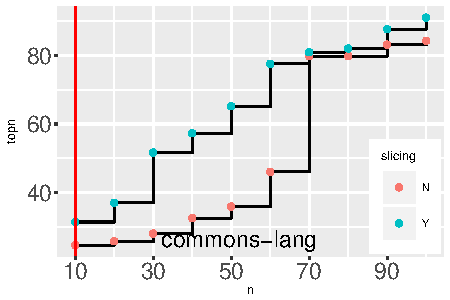
\includegraphics[width=0.25\textwidth]{R/commons-lang-onefailingtest.pdf}}
      &
      \multicolumn{5}{c}{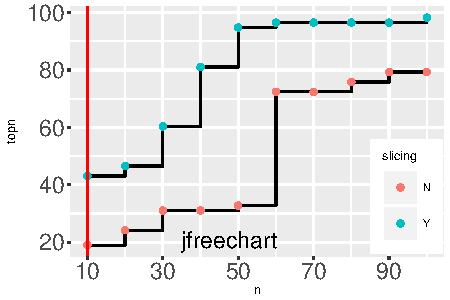
\includegraphics[width=0.25\textwidth]{R/jfreechart-onefailingtest.pdf}}
      &
      \multicolumn{5}{c}{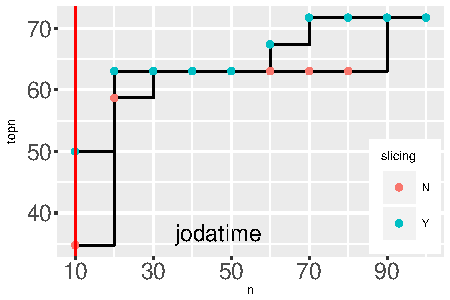
\includegraphics[width=0.25\textwidth]{R/jodatime-onefailingtest.pdf}}\\

      \multicolumn{2}{c}{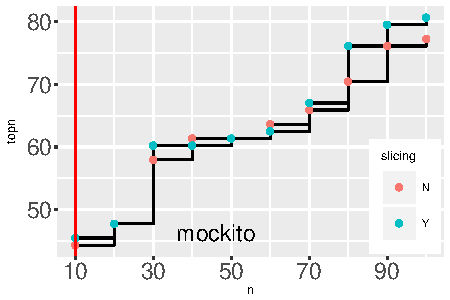
\includegraphics[width=0.25\textwidth]{R/mockito-onefailingtest.pdf}}
      &
      \multicolumn{5}{c}{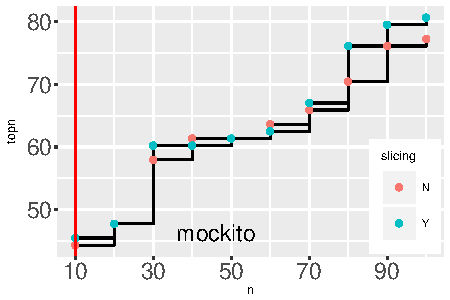
\includegraphics[width=0.25\textwidth]{R/mockito-onefailingtest.pdf}}
      &
      \multicolumn{5}{c}{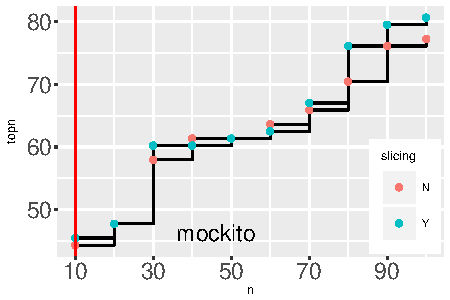
\includegraphics[width=0.25\textwidth]{R/mockito-onefailingtest.pdf}}\\

      \midrule

      \multicolumn{12}{c}{\emph{Filtering statements covered by test(s).}}\\
      \midrule
      \parbox[t]{2mm}{\multirow{4}{*}{\rotatebox[origin=c]{90}{\footnotesize{\sfl}}}}
      & \lang{}     & 33.71 & 41.57 & 49.44 & 52.81 & 60.67 & 84.27 & 94.38 & 95.51 & 96.63 & 98.88 \\
      & \chart{}    & 25.86& 36.21& 36.21& 36.21& 60.34& 75.86& 75.86 & 79.31& 79.31& 79.31 \\
      & \jtime{}       & 43.48 & 63.04 & 65.22 & 69.57 & 71.74 & 71.74 &73.91 & 73.91 & 73.91 & 73.91 \\
      & \mockito{} & 72.09 & 74.42 & 77.91 & 80.23 & 83.72 & 83.72 & 84.88 & 84.88 & 86.05 & 86.05 \\
      \midrule
      \parbox[t]{2mm}{\multirow{4}{*}{\rotatebox[origin=c]{90}{\footnotesize{\comb}}}}
      & \lang{}     & 46.07 & 58.43 & 66.29 & 67.42 & 74.16 & 93.26 & 97.75 & 98.88 & 100.0 & 100.0 \\
      & \chart{} & 51.72& 63.79& 65.52& 86.21& 98.28& 98.28& 98.28& 98.28& 98.28& 98.28 \\
      & \jtime{} & 65.22 & 69.57 & 73.91 & 73.91 & 73.91 & 73.91 & 73.91 & 73.91 & 73.91 & 73.91 \\
      & \mockito{} & 73.26 & 77.91 & 82.56 & 87.21 & 87.21 & 88.37 &91.86 & 94.19 & 95.35 & 95.35 \\
      \midrule

      \multicolumn{2}{c}{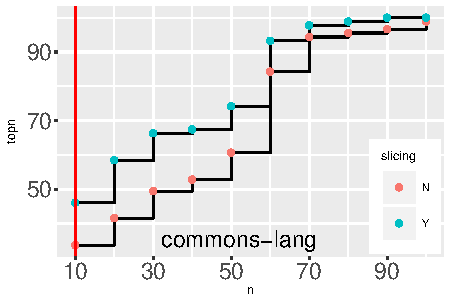
\includegraphics[width=0.25\textwidth]{R/commons-lang-onefailingtest-filtering.pdf}}
      &
      \multicolumn{5}{c}{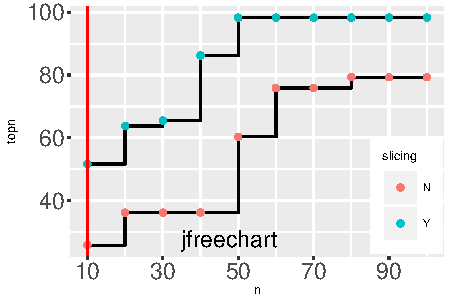
\includegraphics[width=0.25\textwidth]{R/jfreechart-onefailingtest-filtering.pdf}}
      &
      \multicolumn{5}{c}{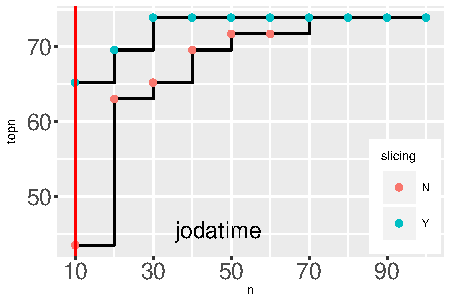
\includegraphics[width=0.25\textwidth]{R/jodatime-onefailingtest-filtering.pdf}}\\

      \multicolumn{2}{c}{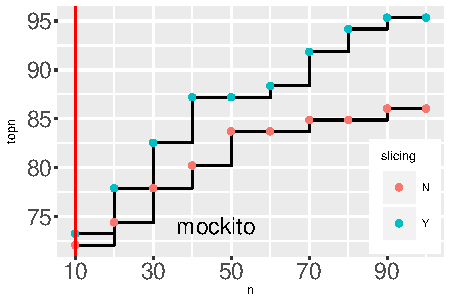
\includegraphics[width=0.25\textwidth]{R/mockito-onefailingtest-filtering.pdf}}
      &
      \multicolumn{5}{c}{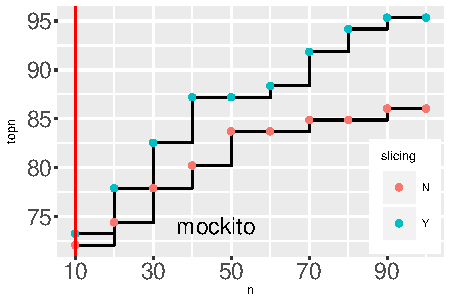
\includegraphics[width=0.25\textwidth]{R/mockito-onefailingtest-filtering.pdf}}
      &
      \multicolumn{5}{c}{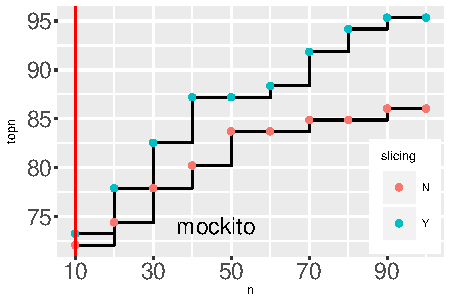
\includegraphics[width=0.25\textwidth]{R/mockito-onefailingtest-filtering.pdf}}\\

      \bottomrule

    \end{tabular}
    \caption{\label{fig:one-failing-test}Top@N, considering one failing test.}
\end{figure*}

\begin{figure*}[!ht]
  \centering
    \begin{tabular}{cl|rrrrrrrrrr}
      \toprule
      & \multicolumn{1}{c|}{Project~\textbackslash{}~LOC}             & 10  & 20  & 30  &  40  & 50  & 60 & 70 &  80 &  90& 100 \\
      \midrule

      \multicolumn{12}{c}{\emph{\textbf{Not} Filtering statements covered by test(s).}}\\
      \midrule
      \parbox[t]{2mm}{\multirow{4}{*}{\rotatebox[origin=c]{90}{\sfl}}}
      &Apache commons-lang     & 25.0  & 27.27 & 29.55 & 38.64 & 43.18
      & 56.82 & 63.64 & 63.64 & 68.18 & 70.45 \\
      &\chart{}       & 50.0  & 68.75 & 75.0  & 75.0  & 75.0  & 87.5  & 87.5  & 87.5  & 93.75 & 93.75 \\
      &Joda-Time       & 23.08 & 38.46 & 46.15 & 46.15 & 46.15 & 46.15
      & 46.15 & 46.15 & 46.15 & 46.15 \\
      &Mockito & 16.67 & 29.17 & 33.33 & 37.5  & 37.5  & 41.67 & 45.83
      & 54.17 & 58.33 & 62.5 \\
      \hline
      \parbox[t]{2mm}{\multirow{4}{*}{\rotatebox[origin=c]{90}{\comb}}}
      &Apache commons-lang     & 36.36 & 50.0  & 56.82 & 59.09 & 63.64
      & 65.91 & 65.91 & 68.18 & 75.0  & 81.82 \\
      & \chart{}       & 68.75 & 81.25 & 93.75 & 100.0 & 100.0 & 100.0 & 100.0 & 100.0 & 100.0 & 100.0 \\
      &Joda-Time       & 30.77 & 46.15 & 46.15 & 46.15 & 46.15 & 46.15
      & 46.15 & 46.15 & 46.15 & 46.15 \\
      &Mockito & 20.83 & 29.17 & 41.67 & 41.67 & 41.67 & 45.83 & 58.33
      & 66.67 & 70.83 & 75.0 \\
      \midrule

      \multicolumn{2}{c}{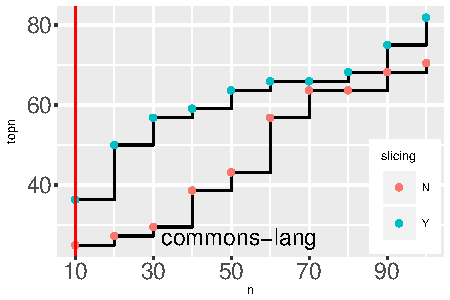
\includegraphics[width=0.25\textwidth]{R/commons-lang-allfailingtest.pdf}}
      &
      \multicolumn{5}{c}{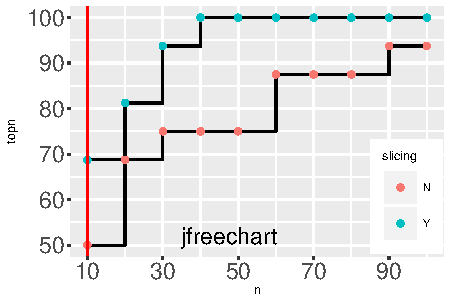
\includegraphics[width=0.25\textwidth]{R/jfreechart-allfailingtest.pdf}}
      &
      \multicolumn{5}{c}{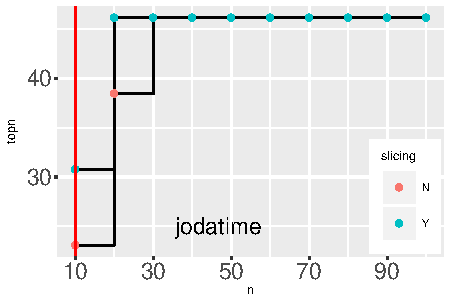
\includegraphics[width=0.25\textwidth]{R/jodatime-allfailingtest.pdf}}\\

      \multicolumn{2}{c}{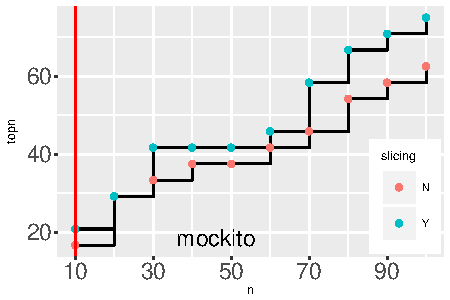
\includegraphics[width=0.25\textwidth]{R/mockito-allfailingtest.pdf}}
      &
      \multicolumn{5}{c}{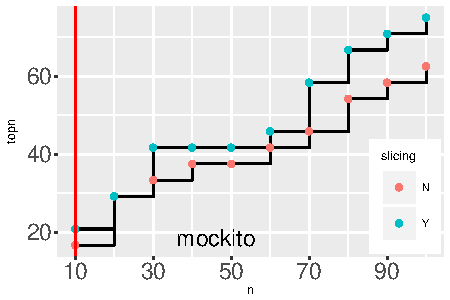
\includegraphics[width=0.25\textwidth]{R/mockito-allfailingtest.pdf}}
      &
      \multicolumn{5}{c}{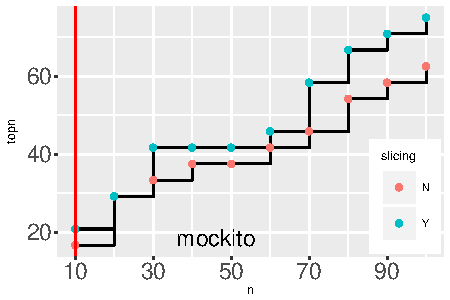
\includegraphics[width=0.25\textwidth]{R/mockito-allfailingtest.pdf}}\\
      \midrule

      \multicolumn{12}{c}{\emph{Filtering statements covered by test(s).}}\\
      \midrule
      \parbox[t]{2mm}{\multirow{4}{*}{\rotatebox[origin=c]{90}{\footnotesize{\sfl}}}}
      & \lang{}     & 36.36 & 45.45 & 59.09 & 63.64 & 70.45  & 79.55 & 88.64 & 90.91 & 93.18 & 97.73 \\
      & \chart{}       & 50.0  & 68.75 & 75.0  & 75.0  & 75.0  & 87.5  & 87.5  & 93.75 & 93.75 & 93.75 \\
      & \jtime{}        & 30.77 & 46.15 & 46.15 & 46.15 & 46.15 & 46.15  & 53.85 & 53.85 & 53.85 & 53.85 \\
      & \mockito{} & 50.0  & 54.17 & 62.5  & 66.67 & 70.83 & 75.0  & 79.17 & 79.17 & 79.17 & 79.17 \\
      \hline
      \parbox[t]{2mm}{\multirow{4}{*}{\rotatebox[origin=c]{90}{\footnotesize{\comb}}}}
      & \lang{}     & 56.82 & 81.82 & 93.18 & 93.18 & 95.45  & 95.45 &95.45 & 97.73 & 100.0 & 100.0 \\
      & \chart{}       & 68.75 & 87.5  & 93.75 & 100.0 & 100.0 & 100.0 & 100.0 & 100.0 & 100.0 & 100.0 \\
      & \jtime{}        & 53.85 & 53.85 & 53.85 & 53.85 & 53.85 & 53.85  & 53.85 & 53.85 & 53.85 & 53.85 \\
      & \mockito{} & 54.17 & 70.83 & 79.17 & 83.33 & 83.33 & 87.5  & 87.5 & 87.5  & 91.67 & 91.67 \\
      \midrule

      \multicolumn{2}{c}{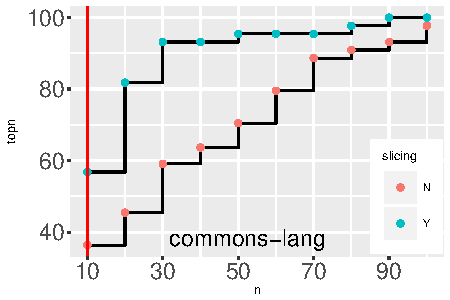
\includegraphics[width=0.25\textwidth]{R/commons-lang-allfailingtest-filtering.pdf}}
      &
      \multicolumn{5}{c}{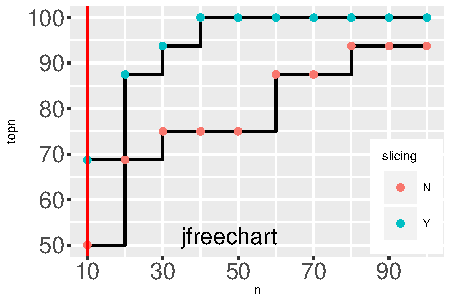
\includegraphics[width=0.25\textwidth]{R/jfreechart-allfailingtest-filtering.pdf}}
      &
      \multicolumn{5}{c}{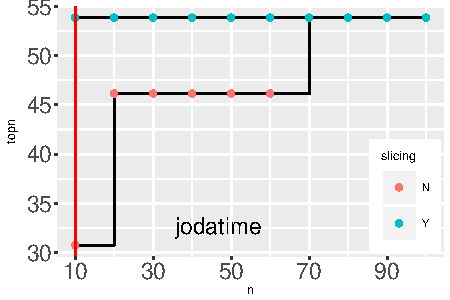
\includegraphics[width=0.25\textwidth]{R/jodatime-allfailingtest-filtering.pdf}}\\

      \multicolumn{2}{c}{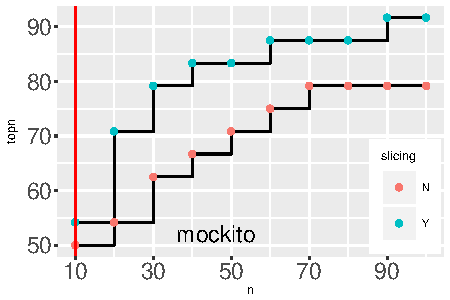
\includegraphics[width=0.25\textwidth]{R/mockito-allfailingtest-filtering.pdf}}
      &
      \multicolumn{5}{c}{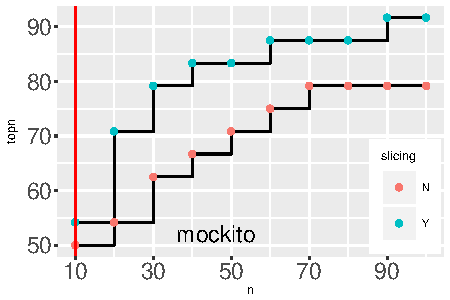
\includegraphics[width=0.25\textwidth]{R/mockito-allfailingtest-filtering.pdf}}
      &
      \multicolumn{5}{c}{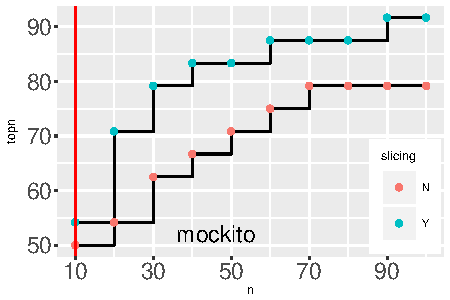
\includegraphics[width=0.25\textwidth]{R/mockito-allfailingtest-filtering.pdf}}\\
      \bottomrule

    \end{tabular}
    \caption{\label{fig:all-failing-test}Top@N, considering all failing test.}
\end{figure*}


%
%We pose the following research questions:

%\textit{RQ1: How frequent are dynamic slices without the bug produced? }
%~\Davino{ XX\% of the results show omission cases, i.e., cases where the fault of the program wasn't present on the generated slice. }

%\textit{RQ2: Are SFL techniques effective on minimizing the effort to manual/automated fault localization?}
%~\Davino{ With the results, we show that it surely isn't. Rank of
%suspiciousness commonly puts the fault at the top 50+ lines of code,
%which isn't practical using manual or automated fault localization, or
%even automated program repair.}

%\textit{RQ3: Can Critical Slicing improve Statistical Fault Localization of real faults in a program?}
%~\Davino{ The results are based on REAL faults (instead of artificial
%ones, which are the basis case of evaluations of techniques involving
%slicing and SFL) presented in Defect4J's data set and show small
%improvements when comparing SFL and DS+SFL.}

\section{Related Work}

\Mar{beware, this is >>NOT<< revised! .........................................................................}

\textbf{Program Slicing}: Most recently related tool is ORBS~\cite{DBLP:conf/scam/BinkleyGHIKY15}. \Fix{...}

Program Slicing~\cite{Weiser:1981:PS:800078.802557} is a technique to
identify program entities (the slice)\Comment{that influence the
  computation of} computationally related to a user-provided point of
interest (the slice criterion).

Similarly, dynamic slicing lacks successful cases of downstream
analyses. The WhyLine debugging assistant~\cite{whyline-website} is an
isolated case of success.


There are some approaches that utilize dynamic slicing and
spectrum-based fault localization (SFL) as fault localization methods.

Ishii and Kutsuna ~\cite{li-huo-chen-zhong-feng-li-2013} proposed a
technique involving dynamic slicing and SFL applied to MATLAB/Simulink
models.The technique consists of iteratively
generating tests that cause an error using satisfiability modulo
theories (SMT) so that the slices generated are distinct from each
other.  For slicing, their technique uses a program dependence graph
(PDG) that express both data and control dependencies between blocks,
so that the slice is built only on blocks that affect a specific line
in the model - \textit{effective blocks}.  Their goal with the slicing
was (1) to keep suspiciousness of a fault maximum if a target model
has only one fault, and (2), to reduce the number of fault candidates
obtained by the slicer.  For this, they utilize only failed test cases
generated with SMT solvers ~\cite{peleska-vorobev-lapschies-2011} to
calculate suspiciousness, as passed test cases might lower the
suspiciousness of a fault.  The calculated suspiciousness is the
number of times that a block belongs to the \textit{effective blocks}
group by the number of total failed test cases.  Although their
experiments and results showed promise with small models, the accuracy
of the technique decreases when applied to models with multiple faults
instead of one, as does the efficiency when exposed to large models,
number of generated tests, sizes of sliced models and so on.



\Fix{...}

\subsection{Automatic Program Repair}
Automated repair techiniques have received considerable attention on
the last decade and consists of three basic steps: fault localization, patch
generation, and patch validation.  Regarding the fault localization
step, Automated Program Repair (APR) tools can be guided by statistical
fault localization techiniques to modify code which most likely
contains the fault. On this section, we will briefly describe some of
these tools.
\Davino { Not necessarily on the paper and not necessarily on a related work section. To be revised/moved/sliced later. }

GenProg\Fix{cite} is a state of the art tool based on genetic
programming to repair defects in off-the-shelf C programs. GenProg's
strategy to fault localization consists of instrumenting the program
so that all lines visited when executing failing test cases are
recorded and used on the genetic search algorithm. The algorithm
involves serching for other parts of the program, considering that a
program that contains an error in one area likely implements the
correct behaviour elsewhere. The tool proved to be effective in
reparing 16 programs involving 1.25 millions LOC, and efficient as the
algorithm search space takes advantage of test case coverage
information, reusing  existing program statements.

Debroy and Wong\Fix{cite} presented a techinique for automatically
fixing faults in a program combining both mutation and statistical
fault localization. Using the Tarantula fault localizer\Fix{cite}, the
techinique focus the top ranked statements in terms of suspiciousness
for the mutation operations. The percentage of statements examined in
search for the fault is based on the total number of statements of the
program, with the 10 percent being a reasonable number on the subject
programs studied.

JAFF\Fix{cite} is a Java automatic repair tool based on evolutionary principles that uses fault localization for ranking the statements in the code in terms of suspiciousness level.
Before searching for the fix, the Java program is translated into a syntax tree composed of nodes related to the top ranked statements being used on the search process.
The tool uses a specific formula to get the number of nodes that will be used on the search based on the number of statements with the same rank of suspiciousness,
with the range between 1 to 20 nodes being used on the cases studied.

SemFix is based on symbolic execution, constraint solving and program synthesis applied to software automatic repair. The tool uses statistical fault localization (SFL) with Tarantula to
obtain the rank of suspiciousness and iteratively takes the most suspicious statement that has not been tried out to be used on the search for a fix. Compared to GenProg, the presented tool
took consideredably less time to find a fix for programs utilizing the same test suites. However, the authors mention that the choice of the SFL techinique could potentially affect the
effectiviness of the tool, particularly with large programs.

SPR\Fix{cite} \Davino{ Fan Long } is based on staged
program repair with condition synthesis. SPR uses fault localization
to identify target statements that will be transformed in search for a
fix on the program. The search space is built with a list of
statements ranked by suspiciousness level, where only the first 200
ranked statements are considered. The authors observed that increasing
the search space to the top 2000 statements would bring additional
repairs, but with a obvious cost of searching a large space.
\Davino { Another tool presented by the same authors is Prophet, which uses the same search space, top 200. }

MintHint \Fix{cite} uses statistical analysis with SFL to rank
statements by their likelihood of being faulty. Given the ranked list,
the tool analysis the top \textit{k} statements, where \textit{k} is a
threshold set by the user, and proceeds with the repair algorithm
assuming the fault can be repaired by changing a single statement.


\Davino { Another set of automatic program repair tools that doesn't use fault localization includes: CodePhage, ClearView, PAR, RSRepair, Kali, and AutoFix, among others. }

\subsection{Dynamic Slicing and Statistical Fault Localization}

Previous works studied the impact of bringing together both dynamic
slicing and statistical fault localization applied to software
debugging.

Lei et al. proposed the use of program slices built with a
dynamic backward slicing approach to defined statistical variables
which can capture the influence of a statement execution on the output
using SFL quantification of suspiciousness to each statement\cite{lei-mao-dai-wang-2012}.

Ishii and Kutsuna proposed a fault localization method with dynamic slicing that iteratively generates failing test cases using Satisfiability Modulo Theories (SMT) solvers to get distinct slices
for each test case. The proposed method was evaluated using MATLAB/Simulink models\cite{ishii-kutsuna-2016}.

Acknowledging the dependencies problem to locate a fault in the probram, Wen\cite{wen-2012} combines the concept of critical slicing, i.e., deleting statements with no contributions to faults,
with statistical fault localization proposing a program slicing spectrum-based software fault localization model.

He et al. proposed a new method to automated fault localization with
CPSS (coverage and program structure slicing)\cite{he-zhang-liu-gao-201}.  Based on program
execution path struture data dependency analysis, the idea is to
extract execution paths streamlined into a complete program dependence
path, reverse data dependence analysis and calculate the defect rate
with state of the art SFL techiniques (i.e., Tarantula).

\subsection{Other}

\Mar{moved to here...revise when possible...}

For example,
dependency tracking alternatives such as
JSlice~\cite{Wang:2004:UCB:998675.999455} and
JavaSlicer~\cite{hammacher-bachthesis-2008} instrument the analyzed
code~\cite{hammacher-bachthesis-2008} or modify
interpreters~\cite{Wang:2004:UCB:998675.999455} to build compact
execution traces.  Then, they process the traces to reconstruct
program states; this step recovers the dependency chains rooted in
points of interest.

ORBS~\cite{Binkley:2014:OLP:2635868.2635893} is a observation-based
slicing method independent of programming language. ORBS deletes
statements in the files of interest and checks whether the test output is
the same as the original
test~\cite{Binkley:2014:OLP:2635868.2635893}.

\Fix{revise? merge?}
Observation-Based Slicing technique, similar to Critical Slicing, is
based on deleting statements that are not relevant to the test case
failure. Although, with this technique is possible to remain the rest
of the system untouched.

%% Acknowledgments
\begin{acks}                            %% acks environment is optional

  %% Commands \grantsponsor{<sponsorID>}{<name>}{<url>} and
  %% \grantnum[<url>]{<sponsorID>}{<number>} should be used to
  %% acknowledge financial support and will be used by metadata
  %% extraction tools.
  This material is based upon work supported by the
  \grantsponsor{GS100000001}{National Science
    Foundation}{http://dx.doi.org/10.13039/100000001} under Grant
  No.~\grantnum{GS100000001}{nnnnnnn} and Grant
  No.~\grantnum{GS100000001}{mmmmmmm}.  Any opinions, findings, and
  conclusions or recommendations expressed in this material are those
  of the author and do not necessarily reflect the views of the
  National Science Foundation.
\end{acks}

%% Bibliography
\bibliography{tmp}

%% Appendix
%% \appendix
%% \section{Appendix}
%% Text of appendix \ldots

\end{document}
